\chapter[Landasan Teori]{\\ Landasan Teori}

\section{Tinjauan Pustaka}
\lipsum[2]

\section{Dasar Teori}
\subsection{Sub Dasar Teori I}
\lipsum[2]

\subsection{Sub Dasar Teori II}
\lipsum[2]

\begin{table}[H]
    \centering
    \caption{Contoh tabel 1}
    \label{t blok}
    \begin{tabular}{|c|l|l|}
        \hline
        \rowcolor[HTML]{C0C0C0} 
        {\color[HTML]{000000} No.} & \multicolumn{1}{c|}{\cellcolor[HTML]{C0C0C0}{\color[HTML]{000000} Nama}} & \multicolumn{1}{c|}{\cellcolor[HTML]{C0C0C0}Fungsi}  \\ \hline
        \rowcolor[HTML]{FFFFFF} 
        1 & \textit{Nama rincian objek yang akan dibahas 1} & Fungsi rincian objek penjelasan 1 \\ \hline
        2 & \textit{Nama rincian objek yang akan dibahas 2} & Fungsi rincian objek penjelasan 2 \\ \hline
        3 & \textit{Nama rincian objek yang akan dibahas 3} & Fungsi rincian objek penjelasan 3 \\ \hline
        4 & \textit{Nama rincian objek yang akan dibahas 4} & Fungsi rincian objek penjelasan 4 \\ \hline
    \end{tabular}
\end{table}


\subsection{Sub Dasar Teori III}
\lipsum[2]

\begin{figure}[H]
    \centering
    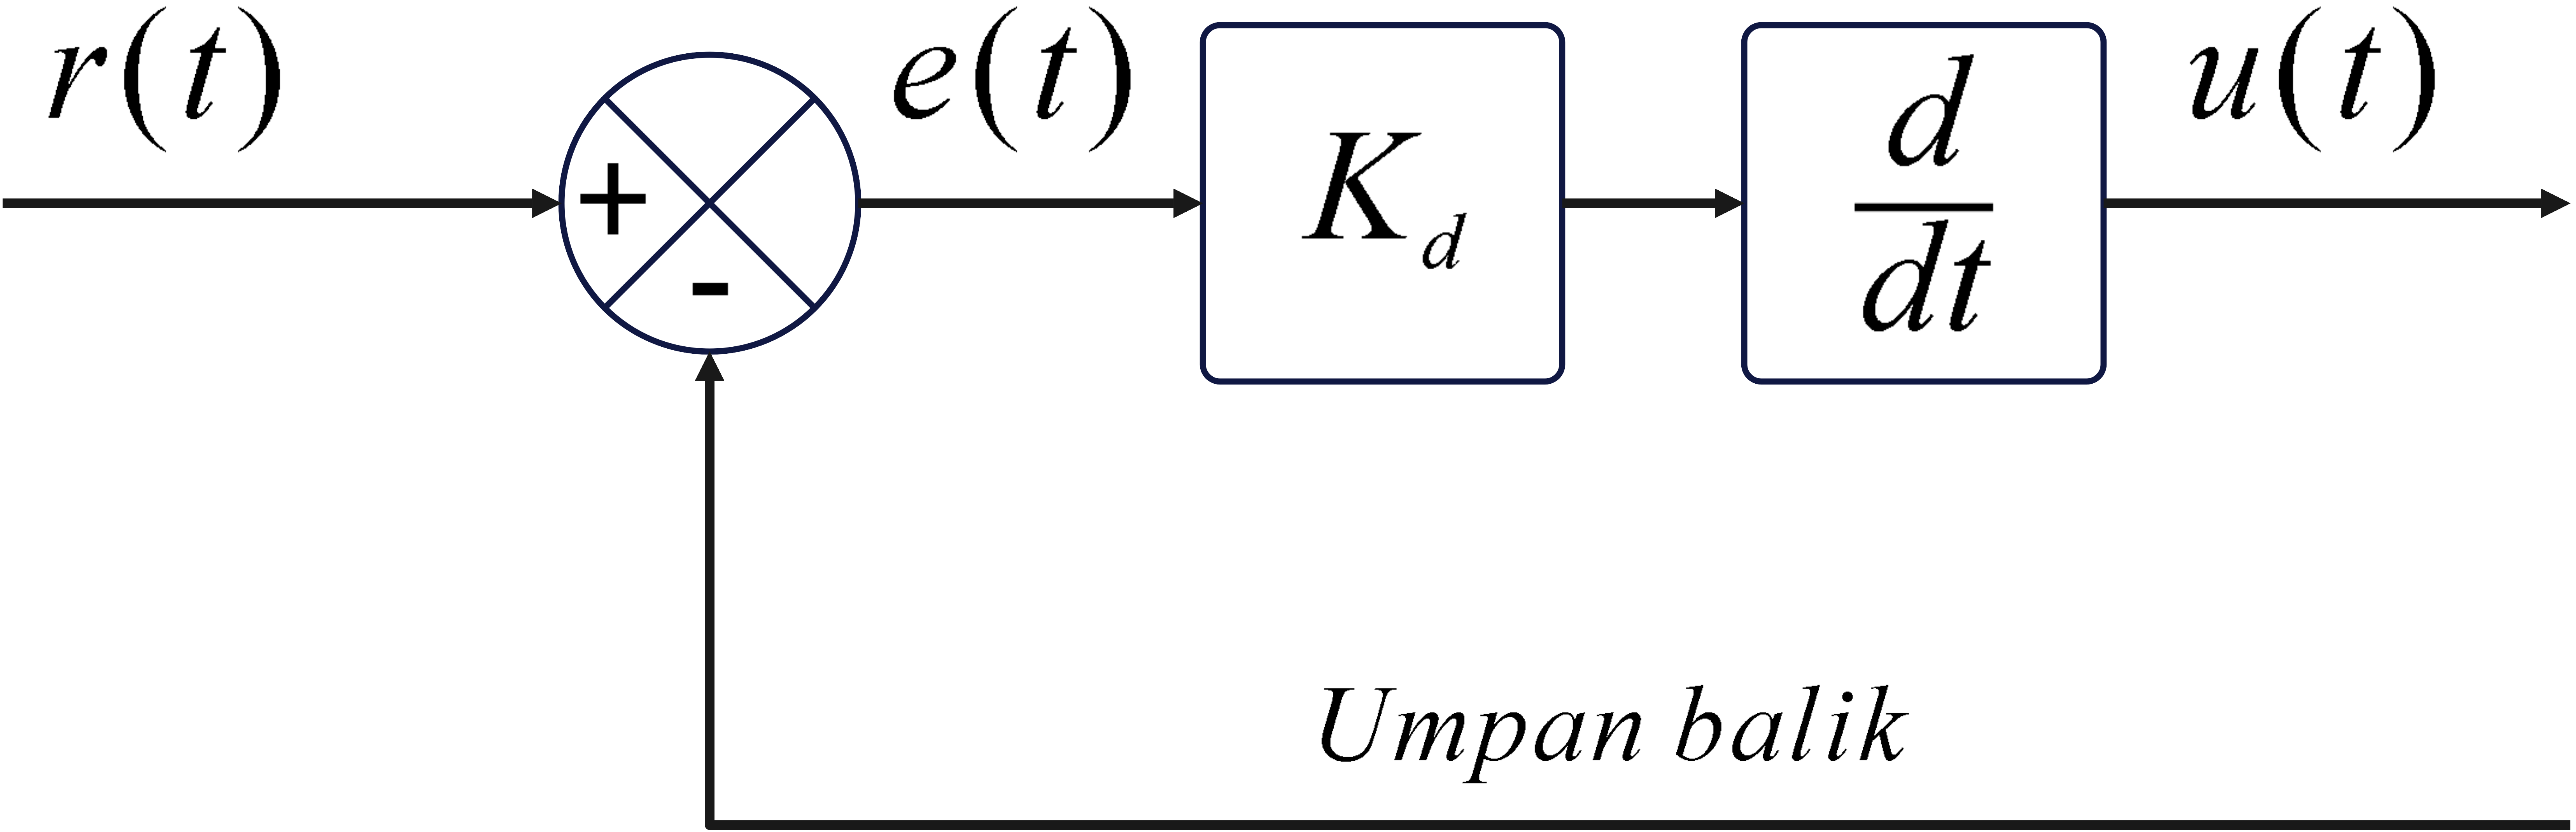
\includegraphics[width=0.8\linewidth]{gambar/diagram.png}
    \caption{Contoh gambar 1}
    \label{gambar1}
\end{figure}

\lipsum[2]

\subsection{Sub Dasar Teori IV}
\lipsum[2]

\section{Hipotesis}
\lipsum[2]

\begin{enumerate}
    \item \lipsum[2][4]
    \item \lipsum[2][4]
    \item \lipsum[2][4]
\end{enumerate}
